\documentclass[12pt]{beamer}
\usetheme{CambridgeUS} % theme

%\titlegraphic{\includegraphics[width=1cm]{logo}}
\title[Application of the P-graph Methodology]{
Application of the P-graph Methodology for Organization-Based Multi Agent System Designs, A graph Transformation approach } 

\author[EL-Houssam]{\textbf {by: Nouar Kherkhachi Houssam \\ \footnotesize Supervised by: Mr Guerrouf Fay\c{c}al}} % auteur
\date{\today} 
\institute[Biskra University]{}




\begin{document}
%\logo{\includegraphics[scale=0.14]{logo}}
\begin{frame}

\begin{center}
	\textbf { University Mohamed khider - Biskra} \\
	\includegraphics[scale=0.7]{logo.png}
\end{center}

\titlepage
\end{frame} 


\begin{frame}
\frametitle{Table of contents}
\tableofcontents
\end{frame} 


% *********************************************************
\section{Introduction} 
\begin{frame}
\frametitle{Introduction} 

\begin{center}
In complex , open environments, agents must be able to reorganize 
 towards the most appropriate organizations to adapt unpredictable environment changes within Multi-Agent Systems .
\end{center}

\end{frame}


\begin{frame}
\frametitle{Overview} 
\begin{center}
Reorganization Types can be seen from two different levels. 
\begin{itemize}
	\item The individual agents level (micro-level) 
	\item The organizational level (macro-level) 
\end{itemize}
\end{center}
\end{frame}
% *********************************************************
\section{Problematic} 
\begin{frame}
\frametitle{Problematic} 
\begin{center}
The problem of our Project is how to get the Optimum structure  
in MaS there's so many framework to use  O-MaSE, OMACS
\end{center}
\end{frame}

% *********************************************************
\section{Definition} 

\begin{frame}
\frametitle{OMACS Framework} 

\begin{columns}
	

	\column{0.45\textwidth}
	 \begin{center}\textbf{OMACS} :
	The Framework of Organization Model for Adaptive Computational  Systems
	\end{center}
	\column{0.5\textwidth} 
	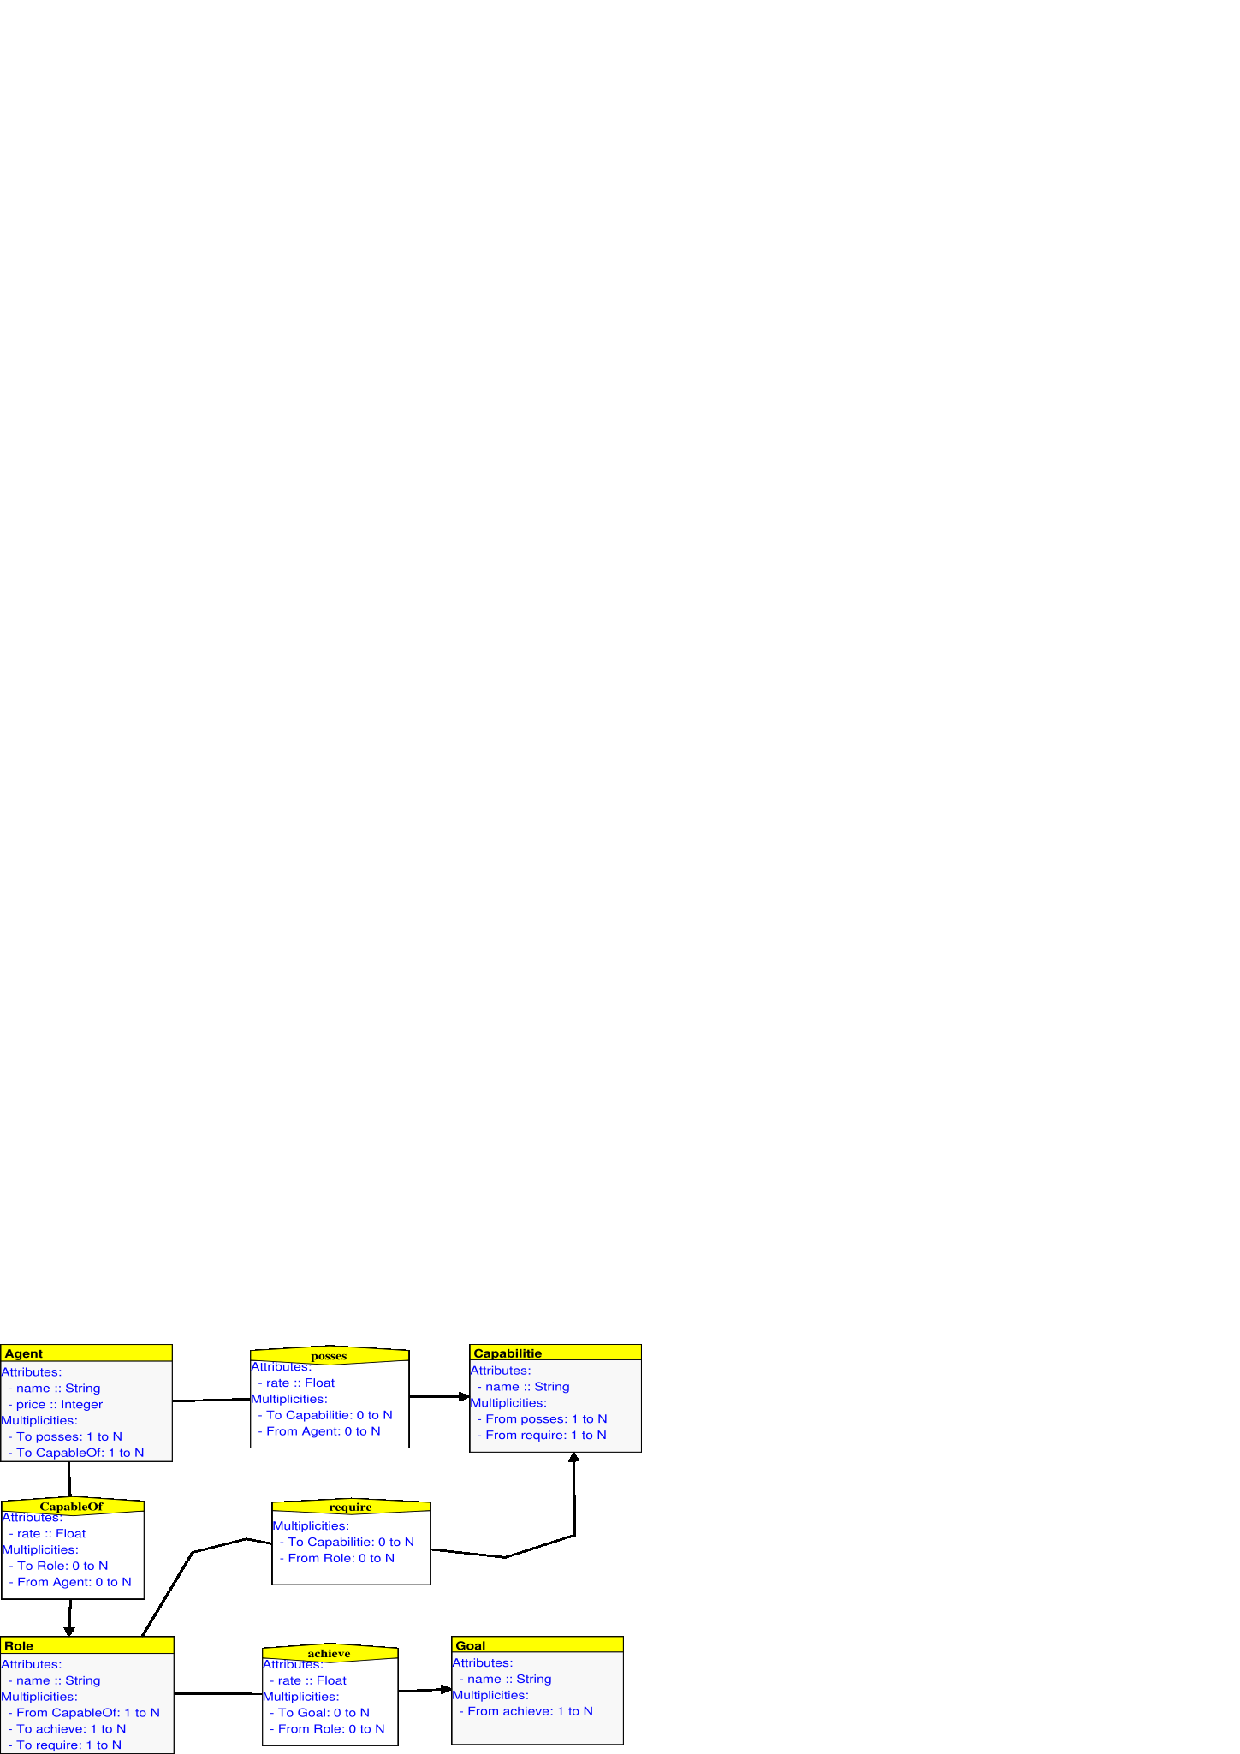
\includegraphics[scale=0.4]{omacs.png}
	
\end{columns}

\end{frame}

\begin{frame}
\frametitle{PNS Framework} 

\begin{columns}
	

	\column{0.45\textwidth}
	 \begin{center}\textbf{PNS} :
	The Framework Which is a directed bigraph, representing 
		the structure of a process system
	\end{center}
	\column{0.5\textwidth} 
	\includegraphics[scale=0.3]{pns.png}
	
\end{columns}

\end{frame}
\section{Graph Transformation}
\begin{frame}
\frametitle{Graتفرق معاكم اذا كنت اكتب بيد الأيسر او الأيمن
ملحوظة : من انا وصغير علمت نفسي على استخدام الأيمن والأيسر حتى من تعطل وحدة استخدم الثانية هههههه لذلك استخدم الاثنينph Transformation} 

\begin{columns}
	
	\column{0.5\textwidth}
	 \begin{center}\textbf{Graph Transformation} :
	or graph rewriting, concerns the technique of creating a new graph out of an original graph
	\end{center}
	\column{0.3\textwidth} 
	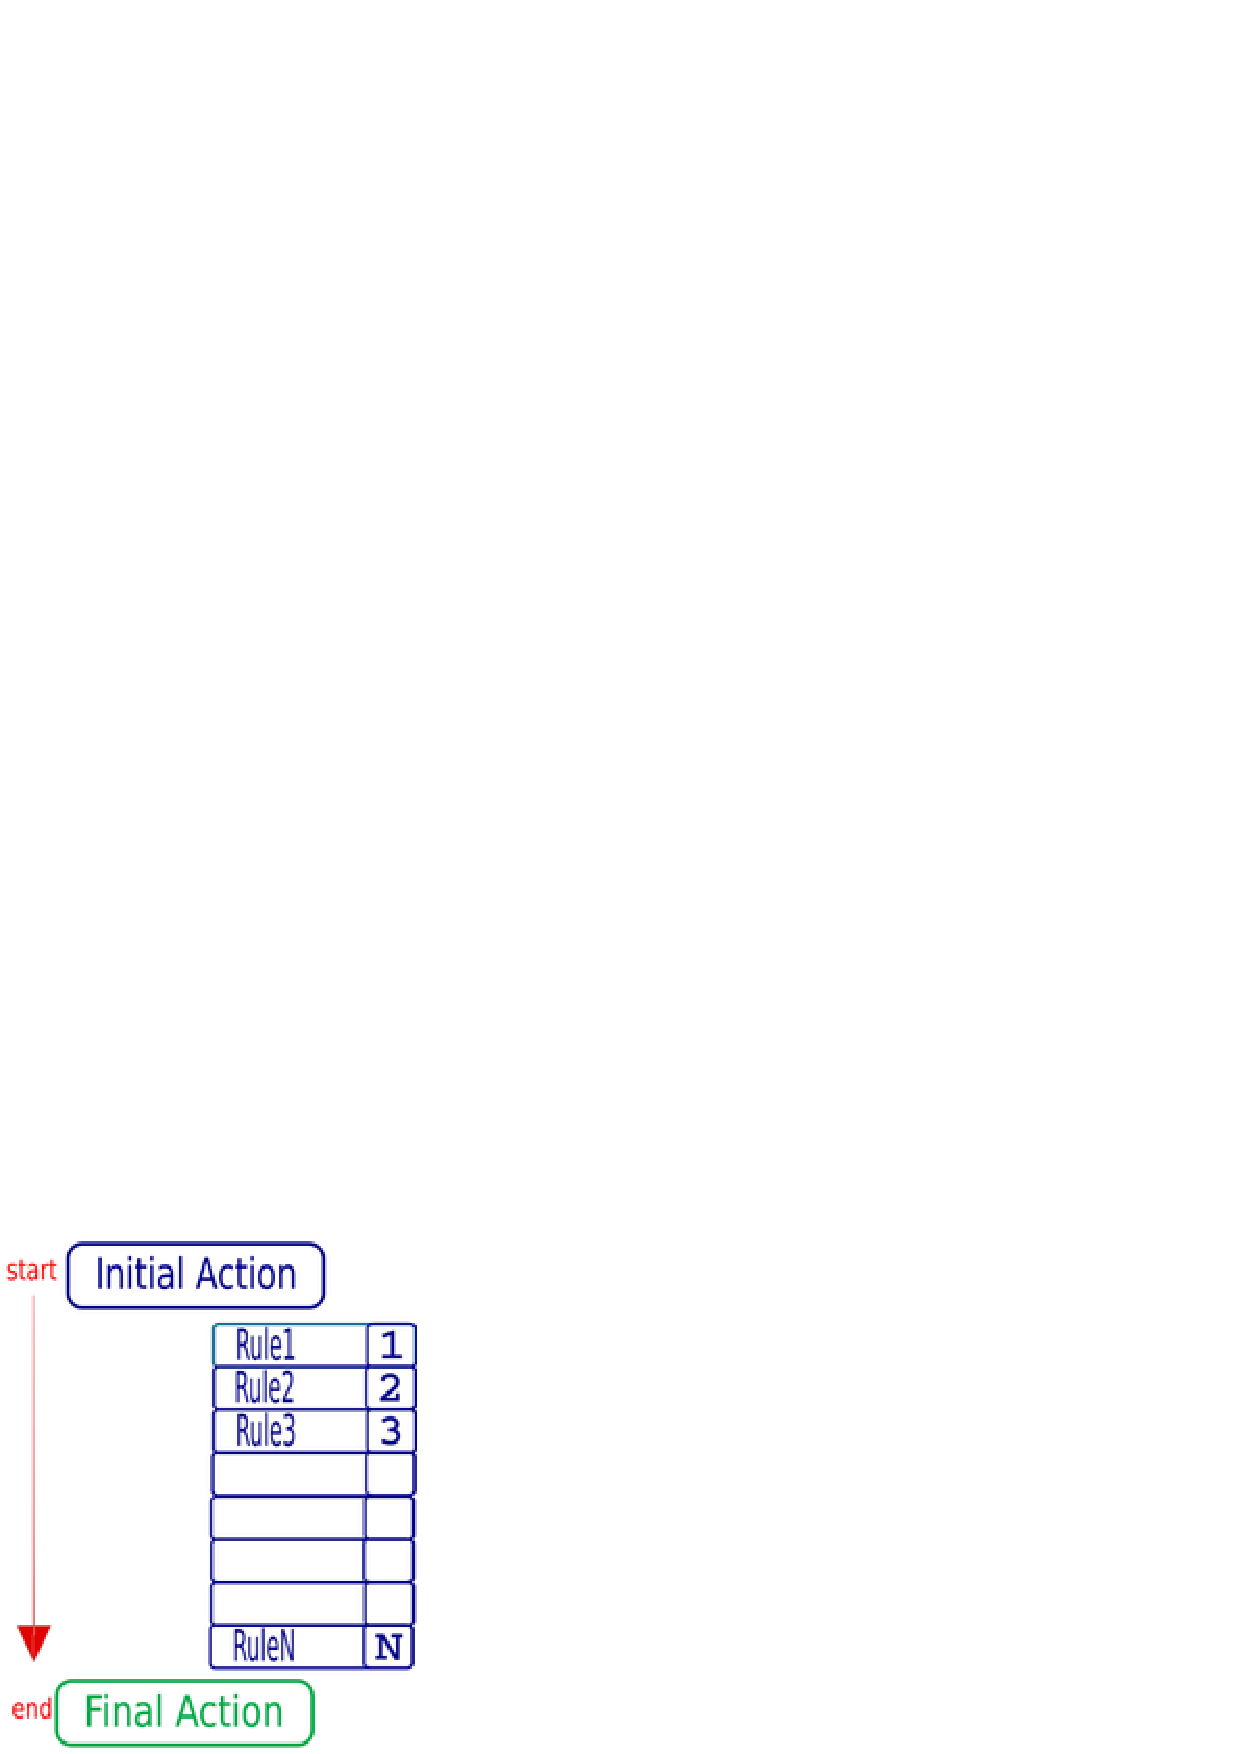
\includegraphics[scale=0.2]{gt.png}
	
\end{columns}

\end{frame}
\begin{frame}
\frametitle{Rule of Transformation} 

\begin{columns}
	
	\column{0.5\textwidth}
	 \begin{center}
	Each rule have two part LHS \& RHS the LHS represent a graph before the transformation and RHS is the graph after we apply the rule.
	\end{center}
	\column{0.5\textwidth} 
	\includegraphics[scale=1.1]{r.png}
	
\end{columns}

\end{frame}
\begin{frame}
\frametitle{Graph Grammar} 
	 \begin{center}	
	\includegraphics[scale=0.7]{cycle.png}
	\end{center}
\end{frame}

\section{Tool AToM3}

\begin{frame}
\frametitle{AToM3 Tool} 
	 \begin{center}	
	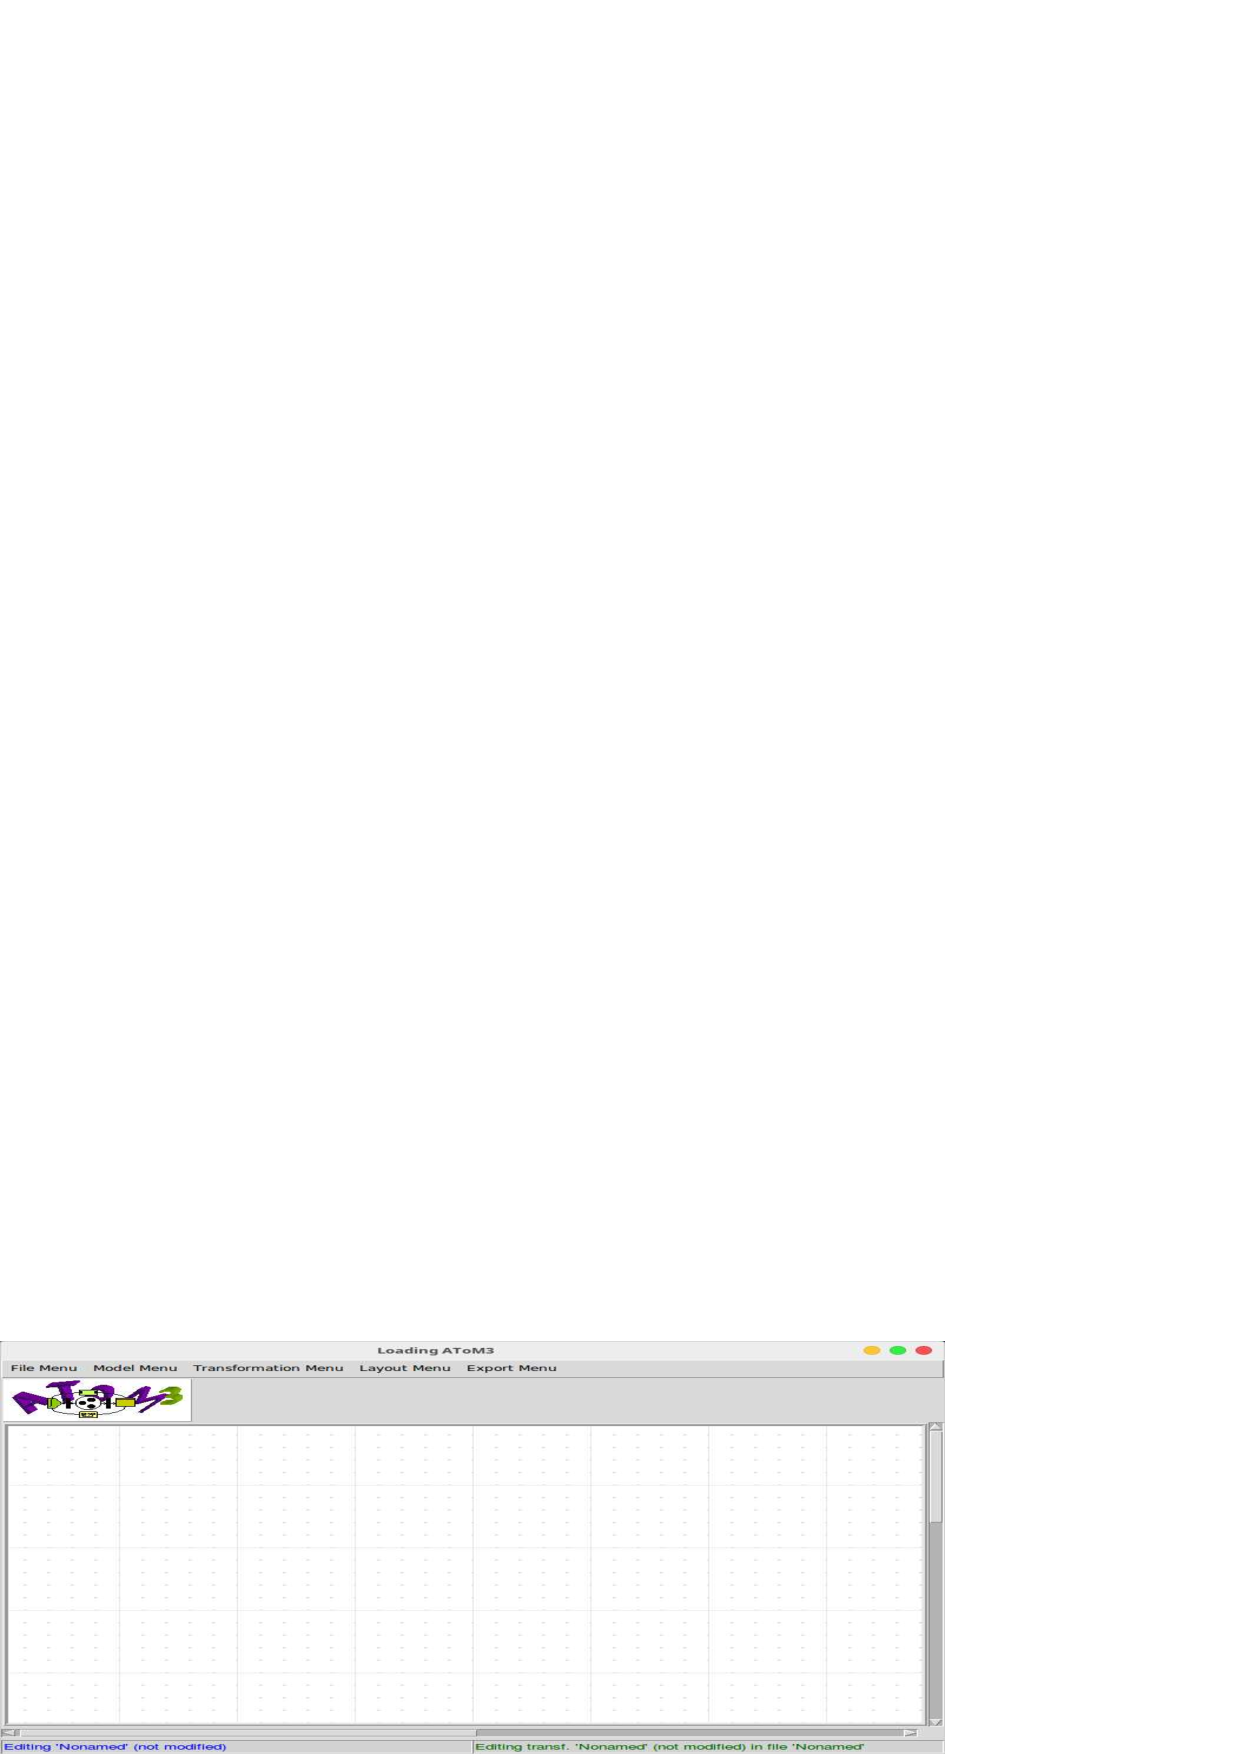
\includegraphics[width=11cm,height=7cm]{atom3.png}
	\end{center}
\end{frame}

 
\begin{frame}
\frametitle{OMACS MetaModel} 
	 \begin{center}	
	\includegraphics[scale=0.5]{omacs_meta}
	\end{center}
\end{frame}
 
\begin{frame}
\frametitle{OMACS example} 
	 \begin{center}	
	\includegraphics[width=10cm,height=6cm]{omacs_ex}
	\end{center}
\end{frame}
 
\begin{frame}
\frametitle{PNS MetaModel} 
	 \begin{center}	
	\includegraphics[scale=0.45]{pns_meta}
	\end{center}
\end{frame}
 
\begin{frame}
\frametitle{PNS example} 
	 \begin{center}	
	\includegraphics[width=10cm,height=6cm]{pns_ex}
	\end{center}
\end{frame}


\section{First Approach (OMACS to PNS)}
\begin{frame}
\frametitle{Rule of Transformation} 

\begin{columns}
	
	\column{0.4\textwidth}
		 \begin{center}	
	\includegraphics[scale=0.5]{L2.png} \\
	left hand side
	\end{center}
	
	\column{0.1\textwidth}
		to
	\column{0.4\textwidth} 
	 \begin{center}	
	\includegraphics[scale=0.5]{R2.png} \\
	right hand side
	\end{center} 
	
\end{columns}

\end{frame}

\begin{frame}

\begin{columns}
	
	\column{0.4\textwidth}
		 \begin{center}	
	\includegraphics[scale=2]{L9} \\
	left hand side
	\end{center}
	
	\column{0.1\textwidth}
		to
	\column{0.4\textwidth} 
	 \begin{center}	
	\includegraphics[scale=1.7]{R9} \\
	right hand side
	\end{center} 
	
\end{columns}

\end{frame}

\begin{frame}
\frametitle{Result from 1st Approach} 

\begin{columns}
	
	\column{0.38\textwidth}
		\begin{center}	
	\includegraphics[scale=0.44]{input} \\
	Source Graph
	\end{center}
	 
	 
	\column{0.38\textwidth} 
	 \begin{center}	
	\includegraphics[scale=0.34]{output} \\
	Target Graph
	\end{center} 
	
\end{columns}

\end{frame}


\section{Second Approach (PNS to XML)}


\begin{frame}
\frametitle{Result from 2nd Approach} 

\begin{columns}
	
	\column{0.38\textwidth}
		\begin{center}	
	\includegraphics[scale=0.3]{output} \\
	Source Graph
	\end{center}
	 
	 
	\column{0.38\textwidth} 
	 \begin{center}	
	\includegraphics[scale=0.19]{erer} \\
	xml file
	\end{center} 
	
\end{columns}

\end{frame}


\section{Tool PGraph Studio}
\begin{frame}
\frametitle{Application of Branch \& Bound } 
	\begin{center}	
	\includegraphics[width=10cm,height=6cm]{optimal.png}
	\end{center}
\end{frame}

\section{Conclusion}
\begin{frame}
\frametitle{conclusion \& perspective} 
\begin{itemize}
\item The definition of two framework (OMACS, PNS)
\item The AtoM3 tool, also the work on these frameworks ( Meta-Model )

\item The first Approach (omacs to pns)
\item The second Approach (pns to xml file)
\item we use the PGraph Studio to optimize the MaS was generated from the 2nd approach \\ 
\textbf{Perspective :} to propose other approach to handle the optimization process instead of PGraph Studio
\end{itemize}
	
\end{frame}

\begin{frame}   
	\begin{center}	
	\emph{\Huge{Thank You}}
	
	\end{center}
\end{frame}

\end{document}